\chapter{Implementacija i korisničko sučelje}
		
		
		\section{Korištene tehnologije i alati}
		
			Za komunikaciju u timu korištene su aplikacije WhatsApp\footnote{\url{https://www.whatsapp.com/}} i Discord\footnote{\url{https://discord.com/}}. UML dijagrami izrađeni su pomoću alata Astah UML\footnote{\url{https://astah.net/products/astah-uml/}}, a zajedno s ostalim materijalima i informacijama u dokumentaciju su uneseni pomoću alata za uređivanje LaTeX dokumenata koji se zove Texmaker\footnote{\url{https://www.xm1math.net/texmaker/}} i beplatne verzije online alata iste vrste Overleaf\footnote{\url{https://www.overleaf.com/}}. Kao sustav za upravljanje izvornim kodom korišten je Git\footnote{\url{https://git-scm.com/}}, a udaljeni repozitorij nalazio se na web platformi GitHub\footnote{\url{https://github.com/}}. 

Kao razvojno okruženje korišteni su Visual Studio Code\footnote{\url{https://code.visualstudio.com/}}, uređivač koda kojie je razvijen od strane kompanije Microsoft za operacijske sustave Windows, Linux i macOS, i IntelliJ IDEA\footnote{\url{https://www.jetbrains.com/idea/}}, integrirano razvojno okruženje (IDE) razvijeno od strane kompanije JetBrains. Backend je realiziran pomoću radnog okvira Node.js\footnote{\url{https://nodejs.org/}} koji omogućuje korištenje jezika JavaScript\footnote{\url{https://www.javascript.com/}} na serverskoj strani aplikacije. API je pisan u jeziku Java\footnote{\url{https://www.java.com/}} uz korištenje radnog okvira Java Spring Boot\footnote{\url{https://spring.io/projects/spring-boot/}} koji ima ugrađenu podršku za zadatke poput upravljanja konfiguracijom, pristupa podatcima u bazi podataka i intergracije sigurnosti u aplikaciju. Aplikacija pristupa MongoDB\footnote{\url{https://www.mongodb.com/}} bazi podataka za čiji je lakši pregled korišten alat MongoDB Compass\footnote{\url{https://www.mongodb.com/products/tools/compass}}. Frontend je raliziran pomoću biblioteke React\footnote{\url{https://react.dev/}}, također poznate kao React.js ili ReactJS, koja omogućuje pisanje HTML koda u JavaScript datotekama što, skupa s modularnom arhitekturom i komponentama koje pruža biblioteka, čini jednostavnim dinamičko generiranje korisničkih sučelja. Za lakše stvaranje nekih komponenti korisnočkog sučelja korišten je radni okvir Bootstrap\footnote{\url{https://getbootstrap.com/}} koji pruža HTML, CSS i JavaScript kod često potrebnih dijelova aplikacije.

Za testiranje API-ja korišten je alat Postman\footnote{\url{https://www.postman.com/}} koji omogućuje slanje različitih vrsta zahtjeva na server. Aplikacija je testirana pomoću alata Selenium WebDriver\footnote{\url{https://www.selenium.dev/documentation/webdriver/}} i JUnit\footnote{\url{https://junit.org/}}, koji omogućuju automatizaciju testiranja web aplikacija pomoću programskog sučelja. Interakcija Selenium WebDrivera s Google Chrome pretraživačem ostavrena alatom ChromeDriver\footnote{\url{https://chromedriver.chromium.org/}}.
			\eject 
		
	
		\section{Ispitivanje programskog rješenja}
			
			\subsection{Ispitivanje komponenti}
			\noindent \textbf{Testni slučaj 1: Provjera addEvent funkcije u Event servisu}
						\begin{itemize}
	
						\item[] \textbf{Ulaz: }
						\begin{packed_enum}
							\item Inicijalizacija događanja
							\item Dodavanje imena "Test Event" događanju 
							\item Pokretanje funkcije \textit{addEvent}
							\item Provjera podudaranja testnog imena s imenom novo nastalog događanja u bazi 
						
						\end{packed_enum}
						\item[] \textbf{Očekivani rezultat: }
						\begin{packed_enum}
							\item Imena će se podudarati
						
						\end{packed_enum}
						\item[] \textbf{Rezultat: }
						\begin{packed_enum}
							\item  Imena se podudaraju
						
						\end{packed_enum}
						\end{itemize}
						
						\begin{figure}[H]
							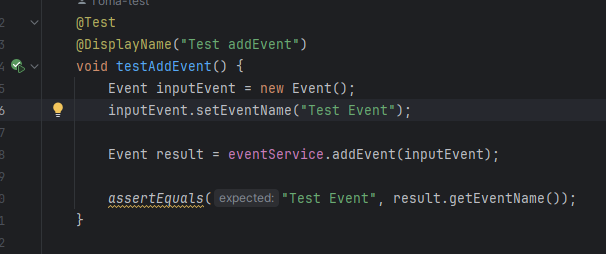
\includegraphics[width=\textwidth]{slike/IKTest1.PNG} %veličina u odnosu na širinu linije
							\caption{Prvi testni slučaj - addEvent}
							\label{fig:IKT1} %label mora biti drugaciji za svaku sliku
						\end{figure}
						\eject
						
						
						
			\noindent \textbf{Testni slučaj 2: Provjera editEvent funkcije u Event servisu}
						\begin{itemize}
	
						\item[] \textbf{Ulaz: }
						\begin{packed_enum}
							\item Inicijalizacija događanja
							\item Dodavanje imena "Original Event Name" i ID-a događanju 
							\item Spremanje događanja pomoću funkcije \textit{addEvent}
							\item Zadavanje novog imena "Updated Event Name" događanju
							\item Pokretanje funkcije \textit{editEvent}
							\item Usporedba uređenog imena sa imenom događanja u bazi
						
						\end{packed_enum}
						\item[] \textbf{Očekivani rezultat: }
						\begin{packed_enum}
							\item Imena će se podudarati
						
						\end{packed_enum}
						\item[] \textbf{Rezultat: }
						\begin{packed_enum}
							\item Događanje ima novo ime koje se podudara "Updated Event Name"
						
						\end{packed_enum}
						\end{itemize}
						
						\begin{figure}[H]
							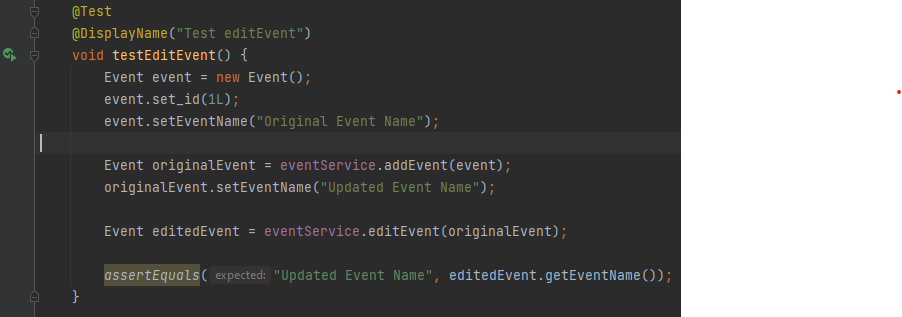
\includegraphics[width=\textwidth]{slike/IKTest2.PNG} %veličina u odnosu na širinu linije
							\caption{Drugi testni slučaj - editEvent}
							\label{fig:IKT2} %label mora biti drugaciji za svaku sliku
						\end{figure}
						\eject
						
						
						
			\noindent \textbf{Testni slučaj 3: Provjera getUserById funkcije u User servisu}
						\begin{itemize}
	
						\item[] \textbf{Ulaz: }
						\begin{packed_enum}
							\item Zadavanje ID-a za pronalaženje
							\item Dohvaća se korisnik s tim ID-em izravno iz baze
							\item Pokretanje funkcije \textit{getUserById} za zadani ID
							\item Usporedba dohvaćenog korisnika izravno iz baze i korisnika dohvaćenog preko funkcije \textit{getUserById}
						
						\end{packed_enum}
						\item[] \textbf{Očekivani rezultat: }
						\begin{packed_enum}
							\item Korisnici su jednaki
						
						\end{packed_enum}
						\item[] \textbf{Rezultat: }
						\begin{packed_enum}
							\item Dohvaćeni korisnici se podudaraju
						
						\end{packed_enum}
						\end{itemize}
						
						\begin{figure}[H]
							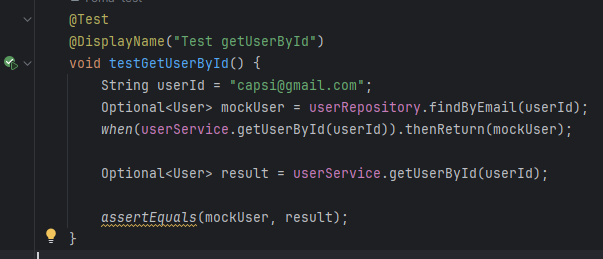
\includegraphics[width=\textwidth]{slike/IKTest3.PNG} %veličina u odnosu na širinu linije
							\caption{Treći testni slučaj - getUserById}
							\label{fig:IKT3} %label mora biti drugaciji za svaku sliku
						\end{figure}
						\eject
						
						
						
			\noindent \textbf{Testni slučaj 4: Provjera getUserById funkcije u User servisu (neuspješno)}
						\begin{itemize}
	
						\item[] \textbf{Ulaz: }
						\begin{packed_enum}
							\item Zadavanje ID-a za pronalaženje
							\item Dohvaća se korisnik s tim ID-em izravno iz baze
							\item Pokretanje funkcije \textit{getUserById} za zadani ID
							\item Usporedba dohvaćenog korisnika izravno iz baze i korisnika dohvaćenog preko funkcije \textit{getUserById}
						
						\end{packed_enum}
						\item[] \textbf{Očekivani rezultat: }
						\begin{packed_enum}
							\item Uspoređuju se dvije prezne vrijednosti jer takav korisnik ne postoji
						
						\end{packed_enum}
						\item[] \textbf{Rezultat: }
						\begin{packed_enum}
							\item Test prolazi jer su obje vraćene vrijednosti prazne
							
						
						\end{packed_enum}
						\end{itemize}
						
						\begin{figure}[H]
							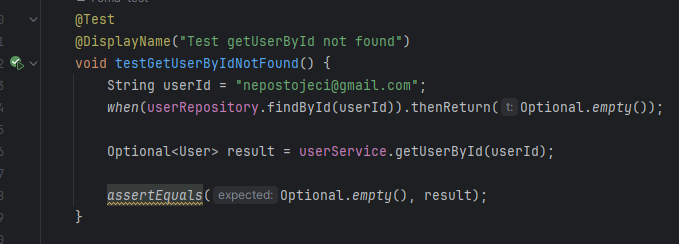
\includegraphics[width=\textwidth]{slike/IKTest4.PNG} %veličina u odnosu na širinu linije
							\caption{Četvrti testni slučaj - getUserById (nepostojeći)}
							\label{fig:IKT4} %label mora biti drugaciji za svaku sliku
						\end{figure}
						\eject
						
						
						
			\noindent \textbf{Testni slučaj 5: Provjera allEvents funkcije u Event servisu}
						\begin{itemize}
	
						\item[] \textbf{Ulaz: }
						\begin{packed_enum}
							\item Dohvaćanje svih događanja izravno iz baze
							\item Pozivanje funkcije \textit{allEvents}
							\item Usporedba dohvaćenih događanja iz baze s dohvaćenim događanjima preko \textit{allEvents} funkcije
						
						\end{packed_enum}
						\item[] \textbf{Očekivani rezultat: }
						\begin{packed_enum}
							\item Dobivena događanja se podudaraju
						
						\end{packed_enum}
						\item[] \textbf{Rezultat: }
						\begin{packed_enum}
							\item Popisi događanja se podudaraju
							
						
						\end{packed_enum}
						\end{itemize}
						
						\begin{figure}[H]
							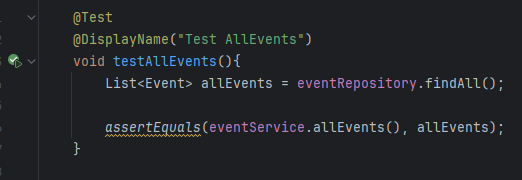
\includegraphics[width=\textwidth]{slike/IKTest5.PNG} %veličina u odnosu na širinu linije
							\caption{Peti testni slučaj - allEvents}
							\label{fig:IKT5} %label mora biti drugaciji za svaku sliku
						\end{figure}
						\eject
						
						
						
			\noindent \textbf{Testni slučaj 6: Provjera getEventById funkcije u Event servisu}
						\begin{itemize}
	
						\item[] \textbf{Ulaz: }
						\begin{packed_enum}
							\item Dohvaćanje događanja preko ID-a izravno iz baze
							\item Pozivanje funkcije \textit{getEventById} za isti ID
							\item Usporedba dohvaćenog događanja iz baze s dohvaćenim događanjem preko \textit{getEventById} funkcije
						
						\end{packed_enum}
						\item[] \textbf{Očekivani rezultat: }
						\begin{packed_enum}
							\item Dobivena događanja se podudaraju
						
						\end{packed_enum}
						\item[] \textbf{Rezultat: }
						\begin{packed_enum}
							\item Događanja se podudaraju
							
						
						\end{packed_enum}
						\end{itemize}
						
						\begin{figure}[H]
							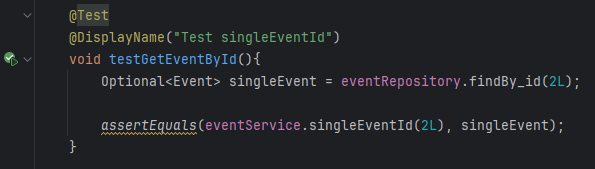
\includegraphics[width=\textwidth]{slike/IKTest6.PNG} %veličina u odnosu na širinu linije
							\caption{Šesti testni slučaj - getUserById}
							\label{fig:IKT6} %label mora biti drugaciji za svaku sliku
						\end{figure}
						\eject
						
				\noindent \textbf{Uspješnost testova - Ispitivanje komponenata}
						\begin{figure}[H]
							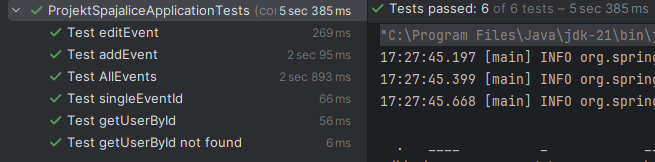
\includegraphics[width=\textwidth]{slike/IKTestovi.PNG} %veličina u odnosu na širinu linije
							\caption{Svi testovi komponenti}
							\label{fig:IKTS} %label mora biti drugaciji za svaku sliku
						\end{figure}
						\eject
						
						
			
			
			
			\subsection{Ispitivanje sustava}
			
				\noindent \textbf{Testni slučaj 1: Provjera \textit{Login} funkcionalnosti (UC3)}
						\begin{itemize}
	
						\item[] \textbf{Ulaz: }
						\begin{packed_enum}
							\item Otvaranje login stranice
							\item Upisivanje podataka za prijavu
							\item Unos podataka u aplikaciju
						
						\end{packed_enum}
						\item[] \textbf{Očekivani rezultat: }
						\begin{packed_enum}
							\item Dobiven novi url kojim se dolazi na prijavljeno sučelje
						
						\end{packed_enum}
						\item[] \textbf{Rezultat: }
						\begin{packed_enum}
							\item Test uspješan
							
						
						\end{packed_enum}
						\end{itemize}
						
						\begin{figure}[H]
							\includegraphics[width=\textwidth]{slike/IsTest1.PNG} %veličina u odnosu na širinu linije
							\caption{Prvi testni slučaj - Login}
							\label{fig:IST1} %label mora biti drugaciji za svaku sliku
						\end{figure}
						\eject
						
						
						
				\noindent \textbf{Testni slučaj 2: Provjera \textit{Login} funkcionalnosti (pogrešni podatci) (UC3)}
						\begin{itemize}
	
						\item[] \textbf{Ulaz: }
						\begin{packed_enum}
							\item Otvaranje login stranice
							\item Upisivanje podataka za prijavu
							\item Unos podataka u aplikaciju
						
						\end{packed_enum}
						\item[] \textbf{Očekivani rezultat: }
						\begin{packed_enum}
							\item Nije dobiven traženi url i javlja se poruka o pogrešno unesenim podatcima
						
						\end{packed_enum}
						\item[] \textbf{Rezultat: }
						\begin{packed_enum}
							\item Test uspješan
							
						
						\end{packed_enum}
						\end{itemize}
						
						\begin{figure}[H]
							\includegraphics[width=\textwidth]{slike/IsTest2.PNG} %veličina u odnosu na širinu linije
							\caption{Drugi testni slučaj - Login (pogrešni podatci)}
							\label{fig:IST2} %label mora biti drugaciji za svaku sliku
						\end{figure}
						\eject
						
						
						
				\noindent \textbf{Testni slučaj 3: Provjera funkcionalnosti kreiranja događanja (UC14)}
						\begin{itemize}
	
						\item[] \textbf{Ulaz: }
						\begin{packed_enum}
							\item Otvaranje login stranice
							\item Prijava
							\item Otvaranje padajućeg izbornika 
							\item Odabir opcije stvaranja događanja
							\item Upisivanje podataka o događanju
							\item Unos podataka u aplikaciju
							
						
						\end{packed_enum}
						\item[] \textbf{Očekivani rezultat: }
						\begin{packed_enum}
							\item Otvaranje \textit{pop up} prozora s potvrdom o stvaranju događanja
						
						\end{packed_enum}
						\item[] \textbf{Rezultat: }
						\begin{packed_enum}
							\item Test uspješan
							
						
						\end{packed_enum}
						\end{itemize}
						
						\begin{figure}[H]
							\includegraphics[width=\textwidth]{slike/IsTest3.PNG} %veličina u odnosu na širinu linije
							\caption{Treći testni slučaj - Kreiranje događanja}
							\label{fig:IST3} %label mora biti drugaciji za svaku sliku
						\end{figure}
						\eject
						
						
						
				\noindent \textbf{Testni slučaj 4: Provjera funkcionalnosti promjene lozinke (UC5)}
						\begin{itemize}
	
						\item[] \textbf{Ulaz: }
						\begin{packed_enum}
							\item Otvaranje login stranice
							\item Prijava
							\item Otvaranje padajućeg izbornika 
							\item Odabir opcije pregleda profila
							\item Klika na gumb za promjenu lozinke
							\item Upisivanje stare i nove lozinke
							\item Unos podataka u aplikaciju
							
						
						\end{packed_enum}
						\item[] \textbf{Očekivani rezultat: }
						\begin{packed_enum}
							\item Otvaranje \textit{pop up} prozora s potvrdom o promjeni lozinke
						
						\end{packed_enum}
						\item[] \textbf{Rezultat: }
						\begin{packed_enum}
							\item Test uspješan
							
						
						\end{packed_enum}
						\end{itemize}
						
						\begin{figure}[H]
							\includegraphics[width=\textwidth]{slike/IsTest4.PNG} %veličina u odnosu na širinu linije
							\caption{Četvrti testni slučaj - Promjena lozinke}
							\label{fig:IST4} %label mora biti drugaciji za svaku sliku
						\end{figure}
						\eject
						
						
						
				\noindent \textbf{Testni slučaj 5: Provjera funkcionalnosti promjene prikaza profila}
						\begin{itemize}
	
						\item[] \textbf{Ulaz: }
						\begin{packed_enum}
							\item Otvaranje login stranice
							\item Prijava
							\item Otvaranje padajućeg izbornika 
							\item Odabir opcije pregleda profila
							\item Klik na gumb za otvaranje prikaza javnog profila
							
						
						\end{packed_enum}
						\item[] \textbf{Očekivani rezultat: }
						\begin{packed_enum}
							\item Dobiven novi url kojim se dolazi na prikaz javnog profila
						
						\end{packed_enum}
						\item[] \textbf{Rezultat: }
						\begin{packed_enum}
							\item Test uspješan
							
						
						\end{packed_enum}
						\end{itemize}
						
						\begin{figure}[H]
							\includegraphics[width=\textwidth]{slike/IsTest5.PNG} %veličina u odnosu na širinu linije
							\caption{Peti testni slučaj - Otvaranje prikaza javnog profila}
							\label{fig:IST5} %label mora biti drugaciji za svaku sliku
						\end{figure}
						\eject
						
						
						\noindent \textbf{Uspješnost testova - Ispitivanje sustava}
						\begin{figure}[H]
							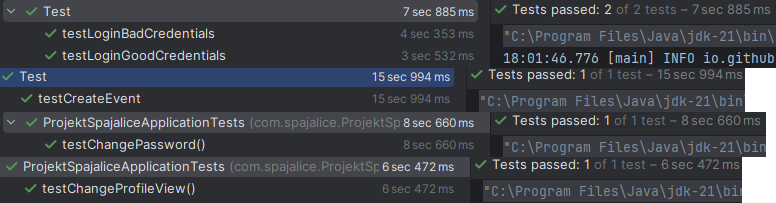
\includegraphics[width=\textwidth]{slike/ISTestovi.PNG} %veličina u odnosu na širinu linije
							\caption{Svi testovi sustava}
							\label{fig:ISTS} %label mora biti drugaciji za svaku sliku
						\end{figure}
						\eject
				
			
		
		
		\section{Dijagram razmještaja}
		Dijagram razmještaja (\ref{fig:DR}) prikazuje fizičku arhitekturu i konfiguraciju razmještaja programskog sustava. Poslužiteljsko računalo sadrži web poslužitelj na kojem je web aplikcaija i poslužitelj baze podataka koji omogućava pristup bazi. Klijent se na sustav spaja pomoću vlastitog osobnog računala koje uspostavlja komunikaciju preko HTTP protokola s poslužiteljskim računalom.  
			
			 \begin{figure}[H]
			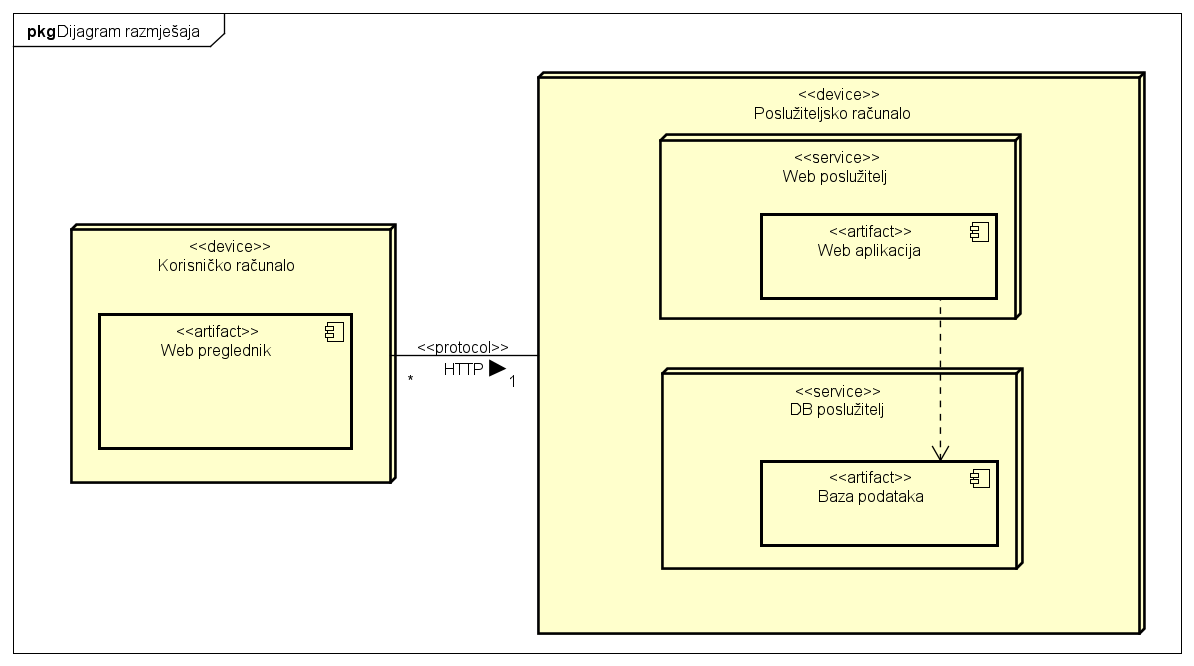
\includegraphics[width=\textwidth]{slike/Dijagram razmjestaja.PNG} %veličina u odnosu na širinu linije
			\caption{Dijagram razmještaja}
			\label{fig:DR} %label mora biti drugaciji za svaku sliku
		\end{figure}
			\eject 
		
		\section{Upute za puštanje u pogon}
		
			\textbf{\textit{dio 2. revizije}}\\
		
			 \textit{U ovom poglavlju potrebno je dati upute za puštanje u pogon (engl. deployment) ostvarene aplikacije. Na primjer, za web aplikacije, opisati postupak kojim se od izvornog kôda dolazi do potpuno postavljene baze podataka i poslužitelja koji odgovara na upite korisnika. Za mobilnu aplikaciju, postupak kojim se aplikacija izgradi, te postavi na neku od trgovina. Za stolnu (engl. desktop) aplikaciju, postupak kojim se aplikacija instalira na računalo. Ukoliko mobilne i stolne aplikacije komuniciraju s poslužiteljem i/ili bazom podataka, opisati i postupak njihovog postavljanja. Pri izradi uputa preporučuje se \textbf{naglasiti korake instalacije uporabom natuknica} te koristiti što je više moguće \textbf{slike ekrana} (engl. screenshots) kako bi upute bile jasne i jednostavne za slijediti.}
			
			
			 \textit{Dovršenu aplikaciju potrebno je pokrenuti na javno dostupnom poslužitelju. Studentima se preporuča korištenje neke od sljedećih besplatnih usluga: \href{https://aws.amazon.com/}{Amazon AWS}, \href{https://azure.microsoft.com/en-us/}{Microsoft Azure} ili \href{https://www.heroku.com/}{Heroku}. Mobilne aplikacije trebaju biti objavljene na F-Droid, Google Play ili Amazon App trgovini.}
			
			
			\eject 